\section{Планирование для дискретного управления}\label{mctssection}

\subsection{Monte-Carlo Tree Search (MCTS)}

Попробуем придумать алгоритм планирования \eqref{planning} в предположении идеального симулятора для MDP с дискретным пространством действий.

Понятно, что для детерминированных MDP с функцией переходов $s' \HM= f(s, a)$, чисто теоретически, мы можем просто построить полное дерево игры. Заведём дерево, в котором каждому узлу будет соответствовать состояние, дугам --- действия, и скажем, что узел, соответствующий $s'$ --- потомок $s$ по дуге $a$, если $s' \HM= f(s, a)$.

У нас есть две проблемы. Во-первых, в сложных MDP такое дерево экспоненциально большое и целиком мы его не построим. Во-вторых, наши MDP, вообще говоря, стохастичны. Мы могли бы ввести много рёбер из $s$, соответствующих одному и тому же действию $a$ и <<подписать>> над каждым вероятности перехода $p(s' \HM\mid s, a)$, однако наша функция переходов $p(s' \HM\mid s, a)$ может быть произвольным распределением, да и вообще пространства состояний $\St$ могут быть в том числе континуальные или очень большие. Поэтому давайте введём понятие дерева чуть-чуть по-другому\footnote{распространены объяснения MCTS в контексте детерминированных MDP, и поэтому про узлы постоянно говорят как про состояния; однако на самом деле ход рассуждений в принципе обобщается на стохастические MDP с тем замечанием, что в силу утверждения \ref{th:planningnotoptimal} в стохастичных средах планирование \eqref{planning} неоптимально.}:

\begin{definition}
\emph{Деревом MDP} с корнем в состоянии $s_0$ будем называть дерево, где каждой дуге соответствует действие $a$; узел на $t$-ом уровне дереве соответствуют плану $a_0, a_1 \dots a_{t-1}$, соответствующему пути от корня.
\end{definition}

Нам нужно продумать эвристики, как сокращать перебор поиска по такому дереву, и как его строить в ситуациях, когда эта задача экспоненциально сложная и у нас ограничены вычислительные ресурсы. Мы сейчас рассмотрим некоторую очень общую схему, как можно такую эвристику строить.

Будем строить дерево MDP с корнем в $s_0$ постепенно. Изначально, на первой итерации, наше дерево пусто --- есть только корень. Узлы дерева будем обозначать красивым символом $\aleph$. Дуги тогда однозначно задаются парой $\aleph, a$, где $\aleph$ --- узел дерева, откуда исходит дуга, $a$ --- действие, которому дуга соответствует. Для каждой дуги $(\aleph, a)$ мы будем также хранить некоторую вспомогательную информацию; самый типичный вариант --- это счётчики прохождения по данной дуге $n(\aleph, a)$ и ценность\footnote{хотя принято обозначать ценности через $V$ или $Q$, это не ценности каких-то состояний: в контексте стохастичных MDP это ценность плана, который привёл нас в это состояние; если угодно, можно обозначить этот счётчик как $Q(s_0, a_0, a_1, a_2 \dots a_t) \HM= \E_{\Traj \mid s_0, a_0, a_1 \dots a_t} R(\Traj)$. Но в детерминированных средах они, конечно же, будут соответствовать оценочным функциям в стандартном понимании.} $Q(\aleph, a)$, скаляр.

Один шаг процедуры \emph{Monte-Carlo Tree Search} (MCTS) заключается в проведении четырёх этапов: Selection, Expansion, Simulation и Update. Введём их по порядку.

\begin{definition}
На шаге \emph{Selection} стартуем в корне, которому соответствует текущее состояние в реальной игре $s_0$. При помощи некоторой стратегии, которую будем называть \emph{TreePolicy}, и которая использует данные на дугах, выбираем действие $a_0$; спускаемся по дереву на уровень глубже по дуге, соответствующей $a_0$, и сэмплируем $s_1, r_1$ из $p(s_1, r_1 \HM\mid s_0, a_0)$. Повторяем процедуру до тех пор, пока не попадём в некоторый лист дерева на уровне $t$. Мы запоминаем (знаем) всю траекторию от корня до листа, то есть фактически выбираем таким образом начало некоторого плана $a_0, a_1 \HM\dots a_{t-1}$ для рассмотрения, и заодно по Монте-Карло генерируем начало возможной траектории, соответствующей этому плану; в результате этой процедуры, мы попадаем в некоторый лист нашего текущего дерева и заодно симулируем для него состояние $s_t$.
\end{definition}

На этом шаге задачей TreePolicy является выбор того плана, для которого мы будем дальше строить дерево. То есть, допустим, мы сидим в некотором узле $\aleph$, не являющемся листом, из которого исходит $|A|$ дуг, и для каждого возможного пути знаем приблизительную оценку качества $Q(\aleph, a)$ и то, сколько раз мы уже пробовали ходить по данной ветке --- $n(\aleph, a)$. Задача этой части эвристики --- найти самый перспективный путь в дереве, используя эти статистики. С одной стороны, нужно искать оптимальный план в той ветке, где оценка качества велика; однако, если по каким-то веткам мы ходили редко, то высока вероятность, что там нам не повезло с сэмплом награды или мы просто недостаточно раскрутили там дерево. Налицо проблема многорукого бандита (см. раздел \ref{sec:bandistssection}); поэтому типичные TreePolicy вдохновлены\footnote{тем не менее, применение бандитов здесь --- тоже эвристика, хотя бы потому, что из-за постепенного раскрытия дерева вдоль каждой ветки <<распределение $p(r \mid a)$>>, из которого приходит дальнейший reward-to-go, меняется.} решениями этой задачи.

\begin{example}[Пример TreePolicy] Воспользуемся UCB-бандитом \eqref{UCB}, формула которого принимает следующий вид:
$$a \coloneqq \argmax_a \left[ Q(\aleph, a) + C \sqrt{\frac{\log n(\aleph)}{n(\aleph, a)}}\right]$$
где $n(\aleph) \coloneqq \sum\limits_a n(\aleph, a)$ --- это счётчик посещений узла, $C$ --- гиперпараметр. Действительно: $n(\aleph)$ --- сколько <<эпизодов игры>> мы провели с этим многоруким бандитом, а $n(\aleph, a)$ --- сколько раз выбирали в этом месте действие $a$. 
\end{example}

\begin{definition}
    На шаге \emph{Expansion} в выбранном на предыдущем этапе листе создаём для каждого действия $a_t \HM\in \A$ по новому листу, соответствующему выбору этого действия: таким образом, мы расширяем дерево вдоль выбранной ветки <<на один шаг вперёд>>.
\end{definition}

\begin{remark}
Если число действий $|\A|$ велико, то имеет смысл определять поднабор действий случайным образом и создавать листы только для него. Тогда этап Selection заканчивается как только, например, TreePolicy сэмплирует действие, для которого ещё не существует дуги.
\end{remark}

\begin{definition}
    Шаг \emph{Simulation} или \emph{Evaluation} заключается в построении некоторой эвристичной оценки reward-to-go для каждого нового построенного на предыдущем шаге листа.
\end{definition}

\needspace{5\baselineskip}
\begin{wrapfigure}{r}{0.5\textwidth}
\vspace{-0.3cm}
\centering
\includegraphics[width=0.5\textwidth]{Images/MCTS.png}
\vspace{-0.3cm}
\end{wrapfigure}

В этом месте, конечно, можно использовать какие-нибудь handcrafted-эвристики, оценивающие очень примерно reward-to-go до конца эпизода (поэтому у этого шага есть второе название Evaluation), но универсальный вариант получить её --- это для каждого $a_t$ просимулировать игру (или несколько) из $s_t, a_t$ до конца эпизода, выбирая действия при помощи некоторой другой стратегии, которую назовём \emph{DefaultPolicy}, и которая уже не может использовать никакой информации в узлах дерева (эти узлы мы ещё просто-напросто не построили). Итого, мы получаем сэмплы reward-to-go для $|\A|$ планов, которые начинаются с $a_0, a_1 \dots a_{t-1}$, на $t$-ом месте действие варьируется, и для каждого варианта у нас есть одна (или несколько) новая Монте-Карло оценка награды.

\begin{example}
Пример типичной DefaultPolicy --- это банально случайная стратегия. 
\end{example}

\begin{definition}
    Шаг \emph{Update} или \emph{Backpropagation}: обновление счётчиков и оценок во всех дугах дерева, по которым мы проходили на данном шаге при помощи полученных на шаге симуляции новых Монте-Карло оценок.
\end{definition}

\begin{example}
Процесс обновления счётчиков прост: в свежераскрытом листе для новых дуг инициализируем $n(\aleph, a) \coloneqq 1, Q(\aleph, a) \coloneqq \hat{V}_a$, где $\hat{V}_a$ --- reward-to-go, полученный на шаге Simulation для действия $a$. Далее, рассмотрим пару $d, a$ где-то в рассмотренной ветке дерева; во-первых, увеличиваем счётчик посещения этой дуги на единицу. Для обновления оценки $Q$ просто учтём новый сэмпл Монте-Карло оценки: мы симулировали награды за шаг, пока шли по дереву, и поэтому можем посчитать reward-to-go до момента прихода в лист. В листе же можно считать, что мы выбирали действие случайным образом, и поэтому усредним все $\hat{V}_a$ по действиям. Таким образом, если $\hat{V}$ --- полученный новый сэмпл reward-to-go, $Q(\aleph, a)$ обновляется как:
$$Q(\aleph, a) \leftarrow Q(\aleph, a) + \frac{1}{n(\aleph, a)}(\hat{V} - Q(\aleph, a))$$
\end{example}

Интуиция, почему это работает: чем больше мы строим дерево, тем меньше зависим от эвристики для этапа Simulation; в пределе после бесконечного числа итераций мы условно построим дерево игры целиком. Чем меньше эта зависимость, тем чаще TreePolicy выбирает хорошие действия. Эвристика из Simulation же лишь указывает на те узлы, куда MCTS быстрее отправится детальнее строить подробное дерево разбора игры, и чем эта эвристика лучше, тем удачнее пройдёт ограниченный перебор.

Вполне можно считать, что расчёт $Q(\aleph, a)$ при помощи Монте-Карло оценок --- это Policy Evaluation, а поиск по дереву при помощи многоруких бандитов --- Policy Improvement.

\subsection{Применение MCTS}

MCTS можно <<предобучить>> перед использованием: проводим много шагов MCTS-процедуры, считая, что корню соответствует $s_0$ (если распределение на начальное состояние стохастично, придётся сэмплировать $s_0$: но тогда, в силу теоремы \ref{th:planningnotoptimal}, мы будем искать план, хороший в среднем для возможных исходов). На каждом шаге MCTS-процедуры ровно один лист в дереве <<раскрывается>> и для каждого пути симулируется одна или несколько игр до конца эпизодов. Полностью дерево для всего MDP мы скорее всего не построим, и однажды придётся остановиться.

Дальше мы хотим нашу стратегию отправить <<играть>> с реальной средой, и тут возможны варианты. Во-первых, мы можем дерево больше не трогать и просто использовать, например, TreePolicy (возможно, с <<выключенным>> эксплорейшном): а то есть, изначально нам дали $s_0$, которое, условно, соответствует корню. Мы выбираем действие при помощи TreePolicy и отправляем его в реальную среду; после этого мы можем в нашем дереве спустится по дуге, соответствующей выбранному действию, и на следующем шаге воспользоваться TreePolicy в этом узле. Однако, во время <<использования>> подобной стратегии нам могут встретиться состояния, для которых в дереве ещё нет узлов; тогда либо придётся выбирать действия случайно, либо проводить новые шаги MCTS-процедуры.

По этой причине, так обычно не делают; считается, что в общем случае, MCTS не строит дерево игры один раз и потом использует его во всех играх, а сама по себе является стратегией выбора действия в данном состоянии: просто долгой и тяжёлой в связи с переборной природой. То есть, перед каждой отправкой итогового действия в среду, нужно провести <<ещё парочку>> итераций MCTS-процедуры. Это означает, что, во-первых, можно вообще предобучения не проводить, а перед каждым выбором действия для реальной среды делать, там, 1000 шагов MCTS-процедуры, а во-вторых, после очередного реального шага, спускаясь на один узел вниз в дереве, мы можем оставлять только поддерево того узла, в который пришли, для оптимизации (наверх по дереву мы никогда не идём --- прошлое уже не изменить).

Итоговое действие для реальной среды не обязательно выбирать при помощи TreePolicy (в нём есть учёт эксплорейшна, который при использовании стратегии нам не нужен). Распространённый вариант следующий: выбирать с большей вероятностью те действия, которые MCTS исследовал чаще всего в ходе всей процедуры:
$$\pi(a_0 \mid s_0) \propto n(\aleph_0, a_0)^T$$
где $T$ --- температура, очередной гиперпараметр.

\begin{remark}
При <<использовании>> стратегии в бою обычно используют жёсткий вариант: $a \coloneqq \argmax\limits_a n(\aleph_0, a)$.
\end{remark}

\begin{algorithm}[label=alg:mcts]{Стратегия MCTS (одна из вариаций)}
\textbf{Вход:} $s_0$ --- текущее состояние реальной среды, $p(s', r \mid s, a)$ --- симулятор, $C$ --- гиперпараметр UCB-бандита, $\aleph_0$ --- корень текущего дерева в памяти с хранением счётков $n(\aleph, a)$ и оценок $Q(\aleph, a)$ в дугах, $K$ --- число шагов, $T$ --- температура.

\vspace{0.3cm}
\textbf{На $k$-ом шаге из $K$:}
\begin{enumerate}
    \item садимся в корень: $\aleph \coloneqq \aleph_0, s \coloneqq s_0$.
    \item инициализируем траекторию симуляции: $\Traj \coloneqq (s_0)$
    \item \textbf{пока $\aleph$ --- не лист:}
        \begin{itemize}
        \item выбираем ветку, куда пойти:
        $$n(\aleph) \coloneqq \sum_a n(\aleph, a)$$
        $$a \coloneqq \argmax\limits_a \left[ Q(\aleph, a) + C \sqrt{\frac{\log n(\aleph)}{n(\aleph, a)}}\right]$$
        \item генерируем $s', r \sim p(s', r \mid s, a)$
        \item сохраняем $a, r, s'$ в $\Traj$
        \item спускаемся по дереву: $\aleph \leftarrow \operatorname{child}(\aleph, a)$, $s \leftarrow s'$
        \end{itemize}
    \item \textbf{для каждого $a \in \A$:}
        \begin{itemize}
        \item создаём узел $\hat{\aleph}$ --- ребёнка $\aleph$ с дугой для действия $a$
        \item симулируем $\Traj_a \sim \pi^{\mathrm{random}} \mid s, a$, где $\pi^{\mathrm{random}}$ --- случайная стратегия
        \item инициализируем $n(\hat{\aleph}, a) \coloneqq 1, Q(\hat{\aleph}, a) \coloneqq R(\Traj_a)$
        \end{itemize}
    \item \textbf{для каждой посещённой дуги $\aleph, a$:}
        \begin{itemize}
        \item считаем $\hat{V}$ --- суммарный reward-to-go в траектории $\Traj$, полученный после посещения данной дуги, где награда после посещения листа оценена как $\frac{1}{|\A|} \sum_{a} R(\Traj_a)$.
        \item $Q(\aleph, a) \leftarrow Q(\aleph, a) + \frac{1}{n(\aleph, a)}(\hat{V} - Q(\aleph, a))$
        \item $n(\aleph, a) \leftarrow n(\aleph, a) + 1$
        \end{itemize}
\end{enumerate}

\vspace{0.3cm}
\textbf{Выход:} стратегия $\pi(a_0 \mid s_0) \propto n(\aleph_0, a_0)^T$
\end{algorithm}

Итого, мы получили очень дорогостоящую по времени, разумную по памяти, но работающую процедуру поиска хороших действий в игре.

\begin{exampleBox}[label=ex:mcts]{}
Попробуем провизуализировать шаг игры при помощи MCTS стратегии. Перед выбором действия будем делать 4 шага MCTS процедуры; выбирать действие для реальной среды будем при помощи $\pi^{\mathrm{MTCS}}(a \HM\mid s) \propto n(\aleph, a)$, где $\aleph$ --- корень дерева.

\begin{center}
\animategraphics[controls, width=\linewidth]{1}{Images/MCTS/MCTS-}{0}{23}
\end{center}
\end{exampleBox}

\subsection{Дистилляция MCTS}

Появляется прекрасная идея: \emph{дистиллировать} MCTS в нейронку. Практически, мы займёмся имитационным обучением с MCTS в качестве эксперта. Для этого мы уже будем проводить этап обучения. Для обучения мы сыграем при помощи вышеописанной стратегии MCTS много игр, и сохраним их траектории\footnote{замечание: траектории именно реальных игр, в которых каждое действие выбиралось в результате, там, 1000 шагов MCTS процедуры, на каждом из которых MCTS делало кучу симуляций при помощи своей DefaultPolicy; эти симуляции внутри MCTS мы нигде не записываем, поскольку нас интересуют только хорошие действия по результатам перебора.} $\Traj$. Далее решаем задачу классификации: пытаемся по состоянию $s$ нейросеткой выдавать действия, которые выбрала бы MCTS. В идеале мы получим стратегию, работающую не хуже MCTS, но при этом скорость прямого прохода по сети будет намного, намного выше.

Схожая альтернатива --- пытаться выдавать нейросеткой-стратегией $p_{\theta}(a \mid s)$ то же распределение, которое выдаёт долгий MCTS перебор; назовём это <<целевое распределение>> $\pi^{\mathrm{MCTS}}(a \mid s)$. Тогда функция потерь выглядит так:
\begin{equation}\label{distill_mcts}
\E_{s} \KL(\pi^{\mathrm{MCTS}}(a \mid s) \parallel p_{\theta}(a \mid s)) = \E_{s} \sum_a \pi^{\mathrm{MCTS}}(a \mid s) \log p_{\theta}(a \mid s) + \const(\theta) \to \min_{\theta},
\end{equation}
где мат.ожидание по $s$ берётся из буфера, из кучи сыгранных при помощи MCTS игр.

И тут возникает желание сделать следующий шаг: если у нас есть нейросеть, которая знает, какие действия в каком состоянии хорошие за счёт моделирования результата MCTS-перебора, может быть мы можем в новой игре воспользоваться ею внутри самого MCTS, использовать эту нейросеть $p_{\theta}(a \mid s)$ для ускорения перебора? Тогда мы наверняка сможем построить ещё более хорошую стратегию, дистиллировать её в нейронку, построить ещё более хорошую стратегию, дистиллировать её в нейронку, и так далее. Итак, появляется идея объединить MCTS с нейросетками.

\subsection{AlphaZero}

В алгоритме AlphaZero\footnote{AlphaZero исторически был обобщением алгоритма AlphaGo для игры в \href{https://ru.wikipedia.org/wiki/Го}{го} как общей процедуры обучения стратегии для произвольной игры с доступным симулятором. Для случая игры двух игроков вроде шахмат и го, для которого она изначально и строилась, предполагается, что в симуляторе за противника играет просто недавняя версия текущей MCTS-стратегии; он также строился для детермированных сред с ненулевой наградой лишь в конце эпизода по типу <<выиграл-проиграл>>, но мы далее опишем сразу чуть-чуть более общую схему.} вводится нейросеть с параметрами $\theta$, принимающая на вход состояние $s$, с двумя головами. Одна выдаёт распределение на действиях $p_{\theta}(a \mid s)$ (<<вспомогательную стратегию>> или <<дистилированную MCTS>>), другая выдаёт скалярную оценку текущего состояния $V_\theta(s)$. Сразу скажем, что $p$ --- лишь вспомогательная стратегия, и хотя ею вполне можно будет пользоваться для игры по итогам обучения, но наша итоговая стратегия всё-таки будет перебирать ходы при помощи MCTS и поэтому будет потенциально лучше. Цель $p_{\theta}(a \mid s)$ --- запоминать с прошлых игр, какие действия были хорошими, ускоряя перебор, а цель $V_{\theta}(s)$ --- запоминать reward-to-go, чтобы не было необходимости проводить симуляции при помощи случайной стратегии на этапе Simulation; вместо симуляции мы теперь просто будем вызывать эту нейросетку.

Итак, за основу алгоритма берётся схема MCTS-стратегии, описанная в алгоритме \ref{alg:mcts}. Как и раньше, в каждом узле $\aleph$ для каждого действия хранится оценка ценности $Q(\aleph, a)$ и счётчик, сколько раз какое действие было попробовано $n(\aleph, a)$; при выборе очередного действия для состояния $s$ повторяется, там, 1600 раз наши четыре этапа MCTS схемы, а каждый эпизод дерево начинает строиться с нуля. 

Изменений в схеме ровно два: на этапе Simulation мы вместо того, чтобы играть случайной стратегией до конца игры, просто воспользуемся нашей моделью $\hat{V}_a \coloneqq V_{\theta}(\hat{s})$ как оценкой дальнейшего reward-to-go (здесь $\hat{s}$ --- симулированное состояние после выбора оцениваемого действия $a$ в листе). Счётчики и скаляры $Q(\aleph, a)$ обновляются как раньше.

Второе изменение --- в формуле TreePolicy, которая принимает следующий вид:
$$a \coloneqq \argmax\limits_a \left[ Q(\aleph, a) + C p_{\theta}(a \mid s) \frac{\sqrt{ n(\aleph)}}{n(\aleph, a) + 1} \right]$$
Здесь $C$ --- гиперпараметр; бонус за исследования немного не похож на UCB-бандита, но имеет примерно тот же смысл (он обратно пропорционален числу выборов действия, а числитель гарантирует, что это слагаемое неограниченно растёт при фиксированном знаменателе и промотивирует выбор любого сколь угодно неоптимального действия рано или поздно). Ключевое изменение --- домножение бонуса на $p_{\theta}(a \mid s)$. Если действие в прошлых играх никогда не выбиралось по итогам перебора, дистилляция в нейросетку приведёт к низкой вероятности $p_{\theta}(a \mid s)$, и такое плохое действие будет выбираться редко. Это позволяет существенно сократить перебор для сред с большим числом\footnote{например, в том же го число доступных действий достигает $19^2$.} действий $|\A|$: в новых состояниях дерева, где все оценки, условно, $Q(\aleph, a) \HM= 0, n(\aleph, a) \HM= 0$, мы вместо случайного тыканья и исследования всех вариантов будем больше опираться именно на те действия, которые показались хорошими нейросетке. Запоминание информации из предыдущих эпизодов обучения направляет раскрытие дерева <<в хорошую область>>.

Как и раньше, результатом работы MCTS является стратегия $\pi^{\mathrm{MCTS}}(a \mid s) \propto n(\aleph_0, a)^T$, где $T$ --- гиперпараметр температуры, $\aleph_0$ --- текущий корень. В ответ на наше действие $a$, сэмплированное из этой стратегии, получаем истинный сэмпл $s'$ из реальной среды и оставляем от нашего дерева лишь поддерево, соответствующее $\operatorname{child}(\aleph_0, a)$.

При помощи такой MCTS-стратегии с текущими параметрами нейросети $\theta$ играем много-много игр и сохраняем записи реальных траекторий; для каждого состояния $s$ запомним $\pi^{\mathrm{MCTS}}(a \mid s)$ и считаем реальный reward-to-go, который обозначим за $z$. Дальше батчами учим $V_\theta$ воспроизводить среднее $z$, минимизируя MSE, а $p_{\theta}(a \mid s)$ --- воспроизводить $\pi^{\mathrm{MCTS}}$ аналогично \eqref{distill_mcts}. Ещё добавлен регуляризатор на параметры, итого:
$$\Loss(\theta) \coloneqq \E_{s} \left[ (z - V_\theta(s))^2 - \sum_a \pi(a \mid s) \log p_{\theta}(a \mid s) + \alpha \| \theta \|^2 \right] \to \min_\theta,$$
где в мат.ожидании $s$ берутся из буфера, $\alpha$ --- гиперпараметр для регуляризации. После многих итераций дообучения нейросети снова играем много игр при помощи MCTS с новыми параметрами нейросетки $\theta$, снова сохраняем записи реальных игр и докидываем их в буфер, и так далее.

В буфере можно хранить в том числе довольно старые игры, поскольку $\pi^{\mathrm{MCTS}}(a \mid s)$ можно считать в некотором смысле <<хорошей>> стратегией даже если $V_\theta(s)$ выдаёт ерунду, а $p_{\theta}(a \mid s)$ условно случайная. Действительно, по мере раскрытия дерева первое <<перестаёт>> использоваться, а второе влияет лишь на исследования внутри самого дерева. Но чем лучше будут эти нейросетки, тем лучше пройдёт MCTS-поиск. Понятно, что $V_{\theta}(s)$, обучаясь на reward-to-go, учит V-функцию для MCTS-стратегии, породившей сэмпл $z$, но ей в таком алгоритме не существенно быть критиком именно самой свежей MCTS-стратегии: ведь в исходной схеме MCTS мы на этапе симуляции так вообще доигрывали игру случайной стратегией.

\begin{example}[AlphaGo Zero]
Основные детали применения данного алгоритма для го можно посмотреть на \href{https://miro.medium.com/max/2000/1*0pn33bETjYOimWjlqDLLNw.png}{этой картинке}.
\end{example}

\subsection{$\mu$-Zero}

Обобщим\footnote{для полноты описания алгоритма, в оригинальной статье введён ещё ряд неприниципиальных изменений в AlphaZero: используется ещё более длинная формула для TreePolicy сразу с несколькими гиперпараметрами, а также вводится обобщение алгоритма на случай частично наблюдаемых сред (см. раздел \ref{sec:PoMDP}).} AlphaZero на случай, когда симулятор нам недоступен. Параметры всех нейросетевых моделей будем обозначать $\theta$, в конечном счёте все части модели будут обучаться end-to-end единой функцией потерь.

На вход стратегии будет приходить реальное состояние среды $s_0$. Оно отправляется в кодировщик: нейросеть $h_{\theta}(s_0)$, которая вернёт латентное представление состояния $\aleph_0$ --- некоторый компактный вещественный вектор. Далее мы для определения стратегии запускаем MCTS-процедуру, однако ей нужен симулятор. В качестве симулятора мы заведём нейросеть $g_{\theta}(\aleph, a)$, которая по данному латентному представлению состояния $\aleph$ и действию $a$ детерминировано выдаст латентное представление следующего состояния $\aleph'$; а также нейросеть $\hat{r}_{\theta}(\aleph, a)$ для моделирования награды за один данный шаг. Поскольку функция $g_{\theta}$ детерминирована, пересчитывать её значение каждый раз, когда MCTS идёт вдоль этой ветки, не понадобится. Нейросети $V_{\theta}$ и $p_{\theta}$ теперь будут тоже принимать на вход компактное латентное представление $\aleph$; это позволит нам внутри дерева запускать их в произвольных узлах.

%Если симулятор $g(\aleph, a, \theta)$ хоть сколько-то похож на реальную динамику среды, MCTS будет выдавать по результатам перебора достаточно хорошую стратегию. 
Осталось понять, как обучать нововведённые функции $g_{\theta}, \hat{r}_\theta, h_{\theta}$. Как и в AlphaZero, соберём датасет из нескольких игр текущей версии модели, и дальше проведём несколько итераций улучшения всех параметров $\theta$. Мы сможем сделать это end-to-end. Возьмём некоторый момент реальной игры с состоянием $s$, reward-to-go с этого момента $z$ и выданной MCTS <<хорошей стратегией>> $\pi^{\mathrm{MCTS}}$. Тогда функция потерь из AlphaZero будет в том числе зависеть от параметров функции $h_{\theta}$:
$$(z - V_\theta(h_{\theta}(s)))^2 - \sum_a \pi^{\mathrm{MCTS}}(a \mid s) \log p_\theta(a \mid h_{\theta}(s)) + \alpha \| \theta \|^2 \to \min_{\theta}$$

Добавить слагаемое для обучения модели функции награды, которая должна воспроизводить награду $r(s, a)$ за один шаг, несложно:
$$\left( r(s, a) - \hat{r}_{\theta}(h_{\theta}(s), a) \right)^2 \to \min_{\theta}$$

Наконец, осталось разобраться с обучением приближения динамики $g_{\theta}$. Тут есть первое соображение: давайте заглянем на один момент в будущее и посмотрим на реальное $s' \HM\sim p(s' \mid s, a)$. Мы могли бы воспользоваться этим сэмплом и явно попросить нашу динамику предсказывать латентное представление будущего: 
$$\|\underbrace{g_{\theta}(h_{\theta}(s), a)}_{\text{\shortstack{предсказанное \\ будущее}}} - \underbrace{h_{\theta}(s')}_{\text{\shortstack{реальное \\ будущее}}}\|_2^2 \to \min_{\theta}$$
Мы так делать не будем (хотя могли бы). Такое слагаемое функции потерь мотивирует латентное представление быть в некотором смысле <<простым>> для предсказания, и эта простота достигается за счёт ухудшения семантического смысла: какие-то важные фичи для $V_\theta, p_\theta$ <<теряются>>, поскольку потеря в лоссе для них меньше, чем потеря в лоссе предсказания усложнённого представления $h_{\theta}(s)$. Нам же важно другое: чтобы латентное представление было <<достаточным>> для предсказания $V_\theta, p_\theta$, будущих наград и хорошей стратегии. Если это достигается, то мы спокойно согласимся как с <<несогласованностью>> латентного описания (когда результат применения модели динамики $g_{\theta}$ не соответствует латентному описанию реального $s'$, хотя всё равно позволяет предсказывать хороший reward-to-go и стратегию для этого $s'$), так и с потерей некоторой информации, несущественной для агента.

Поэтому мы будем обучать $g_{\theta}$ по-другому. Для $s'$ мы знаем целевые переменные для функций $V_\theta, p_\theta, \hat{r}_\theta$. Давайте добавим их лоссы для $s'$, но входное латентное представление для $s'$ получим не при помощи $h_{\theta}(s')$, а при помощи $g_{\theta}(h_{\theta}(s), a)$. То есть пусть $z'$ --- reward-to-go со следующего состояния в реальной игре, $\pi^{\mathrm{MCTS}}(a' \HM\mid s')$ --- результат работы MCTS на следующем шаге $s'$, тогда добавим такое слагаемое в функцию потерь:
\begin{equation*}
(z' - V_\theta(\aleph'_{\theta}))^2 - \sum_{\hat{a}} \pi^{\mathrm{MCTS}}(\hat{a} \mid s') \log p_\theta(\hat{a} \mid \aleph'_{\theta}) + \left( r' - \hat{r}_{\theta}(\aleph'_{\theta}, a') \right)^2 + \alpha \| \theta \|^2 \to \min_{\theta},
\end{equation*}
где $\aleph'_{\theta} \coloneqq g_{\theta}(h_{\theta}(s), a)$.

Заметим, что мы можем взять из буфера целый роллаут длины $K$, и представление для $s^{(k)}$ получать как $k$ преобразований нашей динамикой $g$ представления первого состояния $h_{\theta}(s_0)$; аналогично, для него считать лоссы обучения $V_\theta, p_\theta$ (а также $\hat{r}_{\theta}$). Все выполненные при этом действия следует брать из роллаута, реальной записи игры. Полученные лоссы все суммируются; формальная функция потерь получается следующая:
\begin{equation}\label{muzero}
\sum_{k=0}^K \left[ (z^{(k)} - V_\theta(\aleph^{(k)}_{\theta}))^2 - \sum_{\hat{a}} \pi^{\mathrm{MCTS}}(\hat{a} \mid s^{(k)}) \log p_\theta(\hat{a} \mid \aleph^{(k)}_{\theta}) + \left( r^{(k)} - \hat{r}_{\theta}(\aleph^{(k)}_{\theta}, a^{(k)}) \right)^2 \right] + \alpha \| \theta \|^2 \to \min_{\theta},
\end{equation}
где $z^{(k)}$ --- reward-to-go, начиная с $k$-го шага после рассматриваемого момента времени $s_0$, латентное представление начального состояния определяется кодировщиком $\aleph^{(0)}_{\theta} \HM\equiv \aleph \HM\coloneqq h_{\theta}(s)$, а последующие --- динамикой: $\aleph^{(k)}_{\theta} \HM \coloneqq g_{\theta}(\aleph^{(k - 1)}_{\theta}, a^{(k-1)})$.

Итоговую схему проще представить на картинке:
\begin{center}
    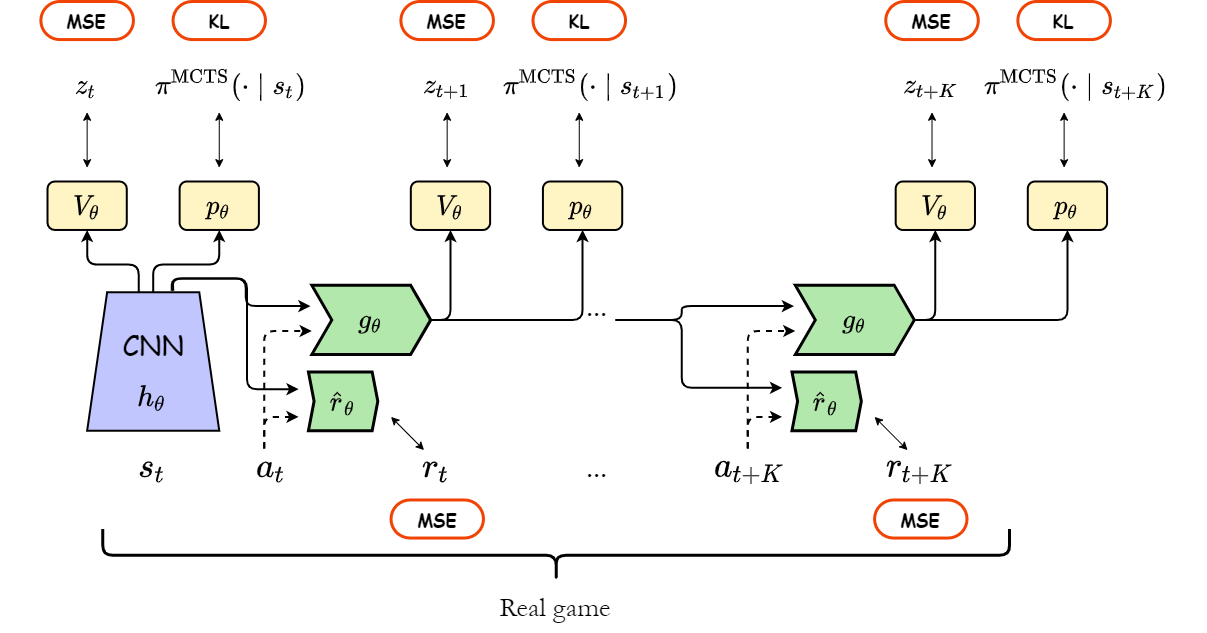
\includegraphics[width=0.9\textwidth]{Images/MuZero.png}
\end{center}

Подумаем, как полученный алгоритм $\mu$-Zero будет обучаться, то есть <<в каком порядке>> будут улучшаться нейросетки. Понятно, что MCTS, в котором динамика среды заменена на необученную нейросетку, ничего разумного выдавать не будет. Однако для обучения модели награды за шаг $r_{\theta}$ в любом датасете у нас всегда будет ground truth, поэтому эта сетка постепенно будет обучаться, и с ходом этого обучения $h_{\theta}$ будет постепенно строить осмысленное латентное представление состояний. Наше приближение $V_{\theta}$, обучающееся на reward-to-go, тоже учится воспроизводить V-функцию <<текущей MCTS-стратегии>>, сколь бы плохой она ни была, и мы помним, что оценочная функция любой стратегии --- это путь к её улучшению. Поскольку мы учимся предсказывать будущие reward-to-go в том числе по преобразованному моделью динамики латентному представлению в слагаемом \eqref{muzero}, модель $g_{\theta}$ научится выдавать такое представление, по которому мы умеем хорошо предсказывать будущие награды. Именно их мы и используем на этапе Simulation в листьях дерева; дерево начнёт ходить в те ветки, где reward-to-go больше, и проводить таким образом policy improvement. Дальше эта более хорошая стратегия будет дистиллироваться в нейронку $p_{\theta}$, а для этого ещё более информативным будет становиться как латентное представление, так и его преобразование моделью динамики.

\begin{remark}
Число итераций на этапе планирования для каждого выбора действий для реальной среды здесь имеет поставить сильно меньше, чем в AlphaZero, поскольку понятно, что перебор с неидеальным симулятором менее осмысленный, чем с идеальным. Тем не менее, универсальность алгоритма $\mu$-Zero противостоит его огромной вычислительной сложности: необходимо делать огромное количество итераций MCTS процедуры, требующей постоянных вызовов нейросетей. 
\end{remark}